% Content specific to importobot-v1.tex

\section{Executive Summary}
\begin{frame}
\frametitle{Bottom Line: What This Means for the Business}
\begin{columns}
\column{0.5\textwidth}
\textbf{Direct Financial Impact:}
\begin{itemize}
    \item Process automation delivers ~150x speed improvement
    \item Estimated \$640K in avoided manual labor costs
    \item Staff time requirements drop by over 99\%
    \item Eliminates human conversion errors entirely
\end{itemize}

\column{0.5\textwidth}
\textbf{Strategic Business Value:}
\begin{itemize}
    \item First automated solution for enterprise test migration
    \item Handles large test suites (10K+ tests) reliably
    \item Significant competitive advantage in the market
    \item Opens doors to new consulting opportunities
\end{itemize}
\end{columns}

\vspace{0.3cm}
\begin{center}
\textcolor{blue}{\textbf{Exceptional ROI with proven technology ready to deploy}}
\end{center}
\end{frame}


\section{Enterprise Migration Case Study}
\begin{frame}
\frametitle{Current System: Large-Scale Test Infrastructure}
\begin{columns}
\column{0.5\textwidth}
\textbf{Existing Test Environment:}
\begin{itemize}
    \item 1,050 tests currently in Zephyr format
    \item Django-based command center for CLI operations
    \item SSH integration for remote system data transfer
    \item 250 tests already automated using custom E2E framework
\end{itemize}

\column{0.5\textwidth}
\textbf{Infrastructure Components:}
\begin{itemize}
    \item pexpect handles CLI command automation
    \item paramiko manages SSH remote operations
    \item Ansible and Terraform provision VMs for testing
    \item 20+ mapped remote systems with automated deployment
    \item Migration goal: standardize on Robot Framework
\end{itemize}
\end{columns}

\vspace{0.3cm}
This mature system provides an excellent foundation for standardization efforts.
\end{frame}

\begin{frame}
\frametitle{Migration Strategy with ImportoBot}
\begin{columns}
\column{0.5\textwidth}
\textbf{Phase 1: Assessment}
\begin{itemize}
    \item Review existing pexpect/paramiko patterns
    \item Map 250 automated tests for conversion
    \item Design Robot Framework architecture
    \item Configure ImportoBot for CLI/SSH operations
\end{itemize}

\column{0.5\textwidth}
\textbf{Phase 2: Automated Conversion}
\begin{itemize}
    \item Train ImportoBot on command structures
    \item Convert SSH operations to Robot libraries
    \item Transform CLI commands to Robot keywords
    \item Migrate VM workflows to Robot test suites
\end{itemize}
\end{columns}

\vspace{0.3cm}
\textbf{Phase 3: Integration}
\begin{itemize}
    \item Integrate CI/CD pipelines with Robot Framework
    \item Convert remaining 800 Zephyr tests using ImportoBot
    \item Deploy unified repository with 1,050 standardized tests
\end{itemize}
\end{frame}

\section{Strategic Growth Plan}
\begin{frame}
\frametitle{Market Expansion Strategy}
\begin{columns}
\column{0.5\textwidth}
\textbf{Near-term Opportunities:}
\begin{itemize}
    \item \textbf{Enterprise Clients}: Zephyr/JIRA migrations (\$2M+ contracts)
    \item \textbf{Consulting Services}: 160x faster delivery = premium pricing
    \item \textbf{Competitive Differentiation}: Only automated enterprise solution
    \item \textbf{Resource Reallocation}: 90\% cost reduction enables growth investment
\end{itemize}

\column{0.5\textwidth}
\textbf{Future Expansion:}
\begin{itemize}
    \item \textbf{New Market Segments}: XML/CSV format clients (4-week implementation)
    \item \textbf{Platform Services}: API-driven SaaS offering
    \item \textbf{AI Integration}: Machine learning for conversion optimization
    \item \textbf{Partnership Opportunities}: Tool vendor integrations
\end{itemize}
\end{columns}

\vspace{0.3cm}
\begin{center}
\textcolor{blue}{\textbf{Flexible design enables rapid market response}}
\end{center}
\end{frame}



\begin{frame}
\frametitle{Implementation Roadmap: 90-Day Value Realization}
\begin{columns}
\column{0.5\textwidth}
\textbf{Phase 1 (Days 1-30): Foundation}
\begin{itemize}
    \item \textbf{System Setup}: Deploy automation platform
    \item \textbf{Team Training}: 2-day technical onboarding
    \item \textbf{Pilot Testing}: 50 test conversions for validation
    \item \textbf{Milestone}: Platform operational, team certified
\end{itemize}

\column{0.5\textwidth}
\textbf{Phase 2 (Days 31-60): Scale}
\begin{itemize}
    \item \textbf{Production Run}: Convert all 800 Zephyr tests
    \item \textbf{Quality Validation}: Automated testing of output
    \item \textbf{Performance Metrics}: Track speed and accuracy
    \item \textbf{Milestone}: Full test suite migrated and verified
\end{itemize}
\end{columns}

\vspace{0.3cm}
\textbf{Phase 3 (Days 61-90): Optimization \& Expansion}
\begin{itemize}
    \item Process additional test formats and optimize workflows
    \item \textbf{ROI Achievement}: \$639,600 cost savings realized
\end{itemize}
\end{frame}

\begin{frame}
\frametitle{90-Day Value Realization Timeline}
\begin{center}
\vspace{-0.2cm}

% Executive-level roadmap with elegant visual design
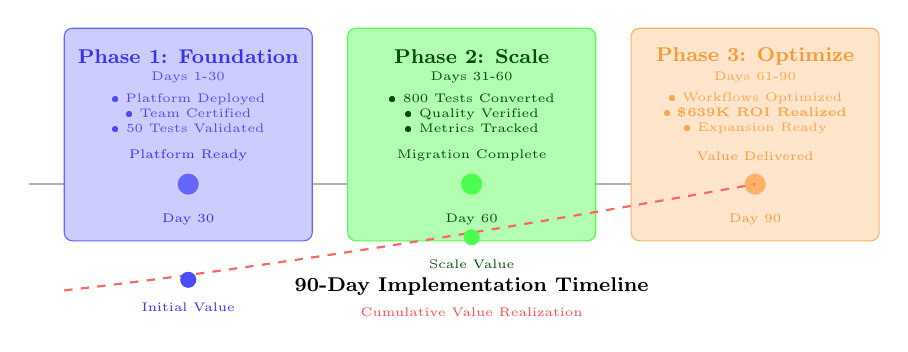
\begin{tikzpicture}[scale=0.9, every node/.style={scale=0.9}]

% Timeline base line
\draw[thick, gray!60] (0,0) -- (12,0);

% Phase blocks with elegant gradients and professional colors
% Phase 1: Foundation (Days 1-30) - Blue gradient (extended)
\filldraw[fill=blue!20, draw=blue!60, rounded corners=3pt] (0.5,-0.8) rectangle (4.0,2.2);
\node[blue!80, font=\footnotesize\bfseries] at (2.25,1.8) {Phase 1: Foundation};
\node[blue!70, font=\tiny] at (2.25,1.5) {Days 1-30};

% Phase 2: Scale (Days 31-60) - Darker Green gradient (extended)
\filldraw[fill=green!30, draw=green!70, rounded corners=3pt] (4.5,-0.8) rectangle (8.0,2.2);
\node[green!30!black, font=\footnotesize\bfseries] at (6.25,1.8) {Phase 2: Scale};
\node[green!30!black, font=\tiny] at (6.25,1.5) {Days 31-60};

% Phase 3: Optimization (Days 61-90) - Orange gradient (extended)
\filldraw[fill=orange!20, draw=orange!60, rounded corners=3pt] (8.5,-0.8) rectangle (12.0,2.2);
\node[orange!80, font=\footnotesize\bfseries] at (10.25,1.8) {Phase 3: Optimize};
\node[orange!70, font=\tiny] at (10.25,1.5) {Days 61-90};

% Timeline markers - elegant circles with phase indicators (positioned to align with curve)
\filldraw[blue!60] (2.25,0) circle (4pt);
\node[below, blue!80, font=\tiny] at (2.25,-0.3) {Day 30};

\filldraw[green!70] (6.25,0) circle (4pt);
\node[below, green!30!black, font=\tiny] at (6.25,-0.3) {Day 60};

\filldraw[orange!60] (10.25,0) circle (4pt);
\node[below, orange!80, font=\tiny] at (10.25,-0.3) {Day 90};

% Key deliverables with executive focus (positioned within extended boxes)
\node[blue!70, font=\tiny, align=center] at (2.25,1.0) {
    • Platform Deployed\\
    • Team Certified\\
    • 50 Tests Validated
};

\node[green!30!black, font=\tiny, align=center] at (6.25,1.0) {
    • 800 Tests Converted\\
    • Quality Verified\\
    • Metrics Tracked
};

\node[orange!70, font=\tiny, align=center] at (10.25,1.0) {
    • Workflows Optimized\\
    • \textbf{\$639K ROI Realized}\\
    • Expansion Ready
};

% Success indicators with icons and metrics (positioned on value curve intersection points)
\node[blue!80, font=\tiny] at (2.25,0.4) {Platform Ready};
\node[green!30!black, font=\tiny] at (6.25,0.4) {Migration Complete};
\node[orange!80, font=\tiny] at (10.25,0.4) {Value Delivered};

% Timeline labels
\node[below, font=\footnotesize\bfseries] at (6.25,-1.2) {90-Day Implementation Timeline};

% Value realization curve - exponential growth curve ending at Day 90
% Start low, slight exponential curve, ending at the Day 90 orange dot
\draw[thick, red!60, dashed] (0.5,-1.5) .. controls (4,-1.1) and (8,-0.4) .. (10.25,0);

% Additional dots positioned ON the value curve at Days 30 and 60
% Day 30 value curve point (blue to match phase above)
\filldraw[blue!70] (2.25,-1.35) circle (3pt);
\node[blue!80, font=\tiny, below] at (2.25,-1.55) {Initial Value};

% Day 60 value curve point (green to match phase above)
\filldraw[green!70] (6.25,-0.75) circle (3pt);
\node[green!30!black, font=\tiny, below] at (6.25,-0.95) {Scale Value};

% The curve terminates at the Day 90 orange dot (10.25,0) - no additional dot needed

\node[red!70, font=\tiny, align=center] at (6.25,-1.8) {Cumulative Value Realization};

\end{tikzpicture}

\vspace{0.3cm}

% Executive summary boxes
\begin{columns}
\column{0.33\textwidth}
\begin{center}
\colorbox{blue!10}{\parbox{0.9\textwidth}{\centering
\textbf{\textcolor{blue!80}{Foundation}}\\
{\footnotesize Platform deployment \& team readiness}
}}
\end{center}

\column{0.33\textwidth}
\begin{center}
\colorbox{green!15}{\parbox{0.9\textwidth}{\centering
\textbf{\textcolor{green!30!black}{Scale}}\\
{\footnotesize Full migration \& validation}
}}
\end{center}

\column{0.33\textwidth}
\begin{center}
\colorbox{orange!10}{\parbox{0.9\textwidth}{\centering
\textbf{\textcolor{orange!80}{Optimize}}\\
{\footnotesize ROI realization \& expansion}
}}
\end{center}
\end{columns}

\end{center}
\end{frame}

\begin{frame}
\frametitle{Investment Analysis: Minimal Risk, Maximum Return}
\begin{columns}
\column{0.5\textwidth}
\textbf{Required Investment:}
\begin{itemize}
    \item \textbf{Platform License}: \$25K one-time setup
    \item \textbf{Professional Services}: \$15K implementation support
    \item \textbf{Training}: \$10K team certification
    \item \textbf{Total Investment}: \$50K compared to \$640K manual effort
\end{itemize}

\column{0.5\textwidth}
\textbf{Resource Allocation:}
\begin{itemize}
    \item \textbf{Implementation Team}: 2 engineers (part-time, 30 days)
    \item \textbf{Ongoing Support}: 1 engineer (maintenance)
    \item \textbf{Infrastructure}: Uses existing development environment
    \item \textbf{Payback Period}: 3 weeks after implementation
\end{itemize}
\end{columns}

\vspace{0.3cm}
\begin{center}
\textcolor{blue}{\textbf{Minimal investment required for substantial returns}}
\end{center}
\end{frame}

